
%(BEGIN_QUESTION)
% Copyright 2015, Tony R. Kuphaldt, released under the Creative Commons Attribution License (v 1.0)
% This means you may do almost anything with this work of mine, so long as you give me proper credit

A wye-connected AC generator has a phase voltage of 7.2 kV, and is connected to a balanced delta-connected load consuming power at a rate of 3.4 MW.  Assuming a power factor of 1 (unity), calculate the following parameters in this polyphase circuit, and draw a sketch of it:

\begin{itemize}
\item{} Line voltage = \underbar{\hskip 50pt} volts
\vskip 5pt
\item{} Line current = \underbar{\hskip 50pt} amps
\vskip 5pt
\item{} Equivalent phase resistance (of load) = \underbar{\hskip 30pt} ohms
\vskip 5pt
\item{} Phase voltage (of load) = \underbar{\hskip 50pt} volts
\vskip 5pt
\item{} Phase current (of load) = \underbar{\hskip 50pt} amps
\vskip 5pt
\end{itemize}

\noindent
Be sure to show all your calculations!

\vfil

\underbar{file i02517}
\eject
%(END_QUESTION)





%(BEGIN_ANSWER)

This is a graded question -- no answers or hints given!

%(END_ANSWER)





%(BEGIN_NOTES)

Important concepts to keep in mind when analyzing three-phase networks is that of {\it series} and {\it parallel} connections: series-connected components must always share the same amount of current, while parallel-connected components must always share the same amount of voltage.  This is why line current and phase current are identical in wye networks: because each phase element is directly in series with each line conductor.  This is why line voltage and phase voltage are identical in delta networks: because each phase element is directly in parallel with a pair of line conductors.

\vskip 10pt

A good problem-solving technique to apply here is to {\it draw a schematic diagram} to organize the figures given to you, and to allow you to more easily see the interconnections of components.

\vskip 10pt

Since we are given the phase voltage of the generator, the total load power, and the Delta-Wye configurations of each, a good place to begin would be calculation of line and load phase voltages.  Since we know a Wye-connected network will have less phase voltage than line voltage (by a factor of $\sqrt{3}$), we know our given generator phase voltage of 7.2 kV will vectorially add to equal a greater line voltage of 12.47 kV.  Our Delta-connected load, by contrast, will exhibit a phase voltage equal to line voltage.  At this point we may also calculate line current, given the relationship between total power, line voltage, and line current: $P_{total} = \sqrt{3} I_{line} V_{line}$.  Solving for $I_{line}$ we get 157.4 amps.

This line current value will split into smaller phase current values for each element of the Delta-connected load, the dividing factor once again being $\sqrt{3}$.  This yields a load phase current of 90.879 A.  In order to calculate phase resistance at the load, all we need to do is divide the total load power by three to arrive at the power dissipated by each single resistor and then apply Joule's Law ($P = I^2 R$ or $P = {V^2 \over R}$) at each resistor to solve for resistance based on power and either voltage (12.47 kV) or current (90.879 A).  Either way we calculate this, the result is the same: 137.22 ohms.


\begin{itemize}
\item{} Line voltage = \underbar{\bf 12,471} volts
\vskip 5pt
\item{} Line current = \underbar{\bf 157.4} amps
\vskip 5pt
\item{} Equivalent phase resistance (of load) = \underbar{\bf 137.22} ohms
\vskip 5pt
\item{} Phase voltage (of load) = \underbar{\bf 12,471} volts
\vskip 5pt
\item{} Phase current (of load) = \underbar{\bf 90.879} amps
\vskip 5pt
\end{itemize}

$$\includegraphics[width=15.5cm]{i02517x01.eps}$$

%INDEX% Electronics review: 3-phase voltage/current/power calculation

%(END_NOTES)


